% 6.4212 final report: Jenga with a mobile iiwa in Drake.
% IEEE conference template (IEEEtran.cls, version 6/27/2024).  Compile in Overleaf (pdfLaTeX).
% Target length (course): ~4500 words for a team of three, not counting figures, references and the AI statement.
% Red [TODO] marks: parts still to write or check.  [OWNER] marks: a teammate writes this part.
% Every number is from docs/DECISIONS.md or the cluster runs; the D-xx / O-x tags point to the entry it comes from.

\documentclass[conference]{IEEEtran}
\usepackage{cite}
\usepackage{amsmath,amssymb,amsfonts}
\usepackage{graphicx}
\usepackage{booktabs}
\usepackage{xcolor}
\usepackage{url}
\newcommand{\todo}[1]{\textcolor{red}{[TODO: #1]}}
\newcommand{\owner}[2]{\textcolor{blue}{[OWNER #1: #2]}}

\begin{document}

\title{Playing Jenga with a Turntable-Mounted iiwa: Rule-Based Block Selection, Camera Perception, and Force Probing in Simulation}

\author{\IEEEauthorblockN{Katie Barkin}
\IEEEauthorblockA{\textit{6.4212, MIT}}
\and
\IEEEauthorblockN{Seetha Senthilnathan}
\IEEEauthorblockA{\textit{6.4212, MIT}}
\and
\IEEEauthorblockN{Mitch Guillaume}
\IEEEauthorblockA{\textit{6.4212, MIT}}
}

\maketitle

% ======================================================================================================
\begin{abstract}
We built a simulated robot that plays Jenga: a KUKA iiwa with a WSG-50 gripper on a turntable base, in Drake, pulls a
block from a six-layer tower and places it on top, one turn after another until the tower collapses. Blocks are taken
by an end-pinch (jaw on the two end faces, for edge blocks) or by a push--pull--regrab sequence (for middle blocks).
We compare a random baseline with a rule-based strategy, and add two layers that work under either: camera perception,
which replaces every block pose the robot uses with an estimate from two simulated RGB-D cameras (hue segmentation and
ICP), and a force probe that nudges a block before taking it. On 100 paired games per condition, the rule-based
strategy places significantly more blocks than random (3.94 vs.\ 3.28 with edges only, $p=0.0013$), a column filter
raises it to 6.27, and perception plays as well as the simulator's ground truth (5.96 vs.\ 5.98, 95\% CI
$-0.21$ to $+0.17$). \todo{one sentence on the probe and the final run once its results are in.}
\end{abstract}

% ======================================================================================================
\section{Introduction}
% Outline: what the task is; why it is interesting for manipulation; what we did; contributions list.
Jenga combines most of what makes contact-rich manipulation hard: the robot has to reach into a structure without
disturbing it, extract a part held in place only by friction, carry it, and set it down precisely enough that the
structure keeps standing. Small errors compound over a game, because each turn leaves the tower in a slightly different
and usually weaker state. The game also has a clear, countable outcome---blocks placed before collapse---which makes it
a good testbed for comparing approaches.

We study the full loop in simulation: a 7-DoF iiwa arm with a parallel-jaw gripper, mounted on a turntable that rotates
the robot around a tower on a raised platform (Fig.~\ref{fig:cameras}). Each turn the robot (i) chooses a block, (ii)
removes it by one of two manipulation methods, and (iii) places it on top. We then ask which choices matter: how the
block is chosen, whether the robot can replace the simulator's privileged state with its own perception, and whether
touching a block first helps decide whether to take it.

Our contributions are:
\begin{itemize}
\item a Drake simulation of the full game with a turntable base, two extraction methods (end-pinch for edge blocks,
push--pull--pedestal regrab for middle blocks) and a reproducible, paired evaluation on a computing cluster;
\item a rule-based selection strategy that beats random play, and a column filter that roughly doubles the number of
blocks placed per game (Sec.~\ref{sec:results});
\item a perception layer (two RGB-D cameras, unique block hues, ICP) that drives every pose the robot uses---including
the block in its own hand---and matches ground-truth play;
\item a force probe that nudges a block before taking it \owner{Mitch/Seetha}{one line};
\item an account of the failure modes we found and how each was traced and fixed (Appendix~\ref{app:log}).
\end{itemize}

% ======================================================================================================
\section{Related Work}
% Outline: robot Jenga; pose estimation (ICP); contact simulation; the course text.  Keep to the closest papers.
\textbf{Robot Jenga.} Fazeli et al.~\cite{fazeli2019} played Jenga with a real robot, learning a hierarchical model
that fuses vision and force to decide how to push blocks. Our force probe asks a related question with a simpler,
threshold-based rule, and our perception uses geometry rather than learning. \todo{add 1--2 more robot-Jenga or
block-extraction papers if we cite them; verify each reference.}

\textbf{Pose estimation.} We estimate each block's pose with the Iterative Closest Point algorithm~\cite{besl1992},
solving each step's rigid alignment in closed form with the SVD~\cite{arun1987}, as in the course's geometric pose
estimation chapter and its reference code~\cite{tedrake_manip}. We add standard outlier rejection, an initial guess from
the robot's own bookkeeping, and a crop around each expected block.

\textbf{Simulation of contact.} The tower stands and slides through Drake's~\cite{drake} hydroelastic contact
model~\cite{elandt2019}. Jenga is unusually sensitive to the contact model: whether a block slides out or drags its
neighbours depends on friction and sub-millimetre gaps, and in our setup the choice of discrete contact solver alone
decided whether a pull dragged the whole layer above (Sec.~\ref{sec:setup}).

% ======================================================================================================
\section{Problem Setup}\label{sec:setup}
% Outline: the game rules we use; the simulation; the robot; how a game is scored; how approaches are compared.
\subsection{The game}
The tower starts with six layers of three blocks (R-04), on a raised platform (R-09). Blocks are real Jenga blocks
scaled by 1.45 to $108.75\times36.25\times21.75$\,mm so they fit the gripper's 110\,mm opening with 3.1\,mm to spare
at each end; the tight margin is in height, 0.875\,mm per side between the fingers and the layers above and below
(D-06). A block may be taken from any layer except the top complete layer and the incomplete one above it (D-09); the
first block of every game is random (R-03). A turn ends in one of: replaced, failed pull, dropped, or collapse; a game
ends at collapse, after two failed turns in a row, or after 10 turns (D-14). The score is the number of blocks placed
before collapse (R-03).

\subsection{Simulation and robot}
One persistent Drake simulator runs each game, built by hand in the course's problem-set style (D-03). Contact is
hydroelastic~\cite{elandt2019} with Drake's ``lagged'' discrete approximation: with the default SAP solver a pull of one
bottom block dragged the whole layer above out with it (70\,mm of a 100\,mm pull) although that layer rested only 0.42\,N
on the pulled block and 3.11\,N on its neighbours; with ``lagged'' the same plan moved no other block more than 0.2\,mm
(D-10). The arm, fingers and base are PD-controlled joints of the plant, with gravity
off for the arm links (an ideal gravity-compensated arm) (D-19); hand-velocity commands are converted to joint
velocities by differential inverse kinematics and integrated in discrete 1\,ms substeps (D-24). The course's continuous
integrator was stepped by the simulator, which also stops at every replay frame, so recording a game changed its result
(the same trial placed 6 blocks without a replay and 4 with); the discrete one makes replays exact (to 0.01\,mm). The robot stands on a
turntable: one revolute joint about the vertical axis through the tower, 0.95\,m out, so it reaches the tower from a
set of stations around it (D-02). The hand stays level throughout (R-10).

\subsection{Evaluation}
Each condition plays the same numbered trials; trial $i$ fixes the first block and the friction draw with seed $1000+i$
(D-15), so two conditions on the same trial start identically and can be compared game by game. We compare blocks per
game with the paired Wilcoxon signed-rank test (Holm-corrected when several comparisons are planned), early failures
(games with $\le$1 block) with McNemar's exact test, and equivalence with two one-sided tests. Measures were fixed
before each confirmation run, and every chosen setting was confirmed on fresh trials it was not tuned on. A collapse is
any block other than the moved one moving more than 20\,mm (D-12). Hidden from every strategy: per-block friction and
contact forces (R-05).

% ======================================================================================================
\section{Approach}\label{sec:approach}
% Outline: A. extraction methods; B. placing; C. strategies; D. perception; E. force probe.
\subsection{Extraction methods}
\textbf{End-pinch (edge blocks).} The hand approaches level from the side, closes on the block's two end faces and
slides it out sideways (R-06). The robot faces the block's long side, so each layer is reachable only from the two
stations across it (D-08). Our \texttt{plan\_pull} (Katie) starts 100\,mm back along the reach axis with the
fingers open, moves in so the pads sit at the block's mid-height, closes in two steps (the second held 1\,s so the
fingers finish closing before the hand moves), pulls straight back, and lifts 300\,mm. Pad height is critical: an early
version used half the block's \emph{width}, 7.25\,mm too high against the 0.875\,mm margin. Because a waypoint's finger
command takes effect only on the next leg, we gave each waypoint an optional duration, so a closing step can be held
in place (D-04). The pull-out is fast, 100\,mm in 0.1\,s: at 1.0\,s a layer-4 pull collapsed a fresh six-layer tower,
at 0.1\,s layer-3 and layer-4 pulls moved the tower only 1.6 and 2.5\,mm (D-23); a fast pull gives friction less time
to drag the layers above and below. The squeeze ($L-2\times$\texttt{FINGER\_SQUEEZE\_M}) dates from the layer-drag
diagnosis, when we doubled it; a 6\,s pull, a half-out-and-back pull and a 10\,mm lower grasp did not help there---the
contact model did (Sec.~\ref{sec:setup}). We kept it for a firmer grip, so the block does not slip in the pads
during the fast pull-out and the carry. The 100\,mm approach lets the open fingers clear the block's ends and its
neighbours before moving straight in, and the 300\,mm lift carries the held block clear of the tower top before the base
turns; both were round, safe first choices that never needed changing.

\textbf{Push (middle blocks).} A middle block cannot slide past its neighbours, so the robot faces its end, pushes it
0.4 block lengths out the far side, turns to the opposite station, grips the protruding end and pulls it out (D-21).
Developing it (Katie) took most of a week of tracing why the pull dragged the tower. A fast ``tablecloth'' pull still
moved the worst block 13--16\,mm; contact-force readouts showed the block above (block 4) loading the pulled block
more than its other supports and pushing its neighbour off along the pull direction; the squeeze was the main lever
(worst block 194\,mm at a squeeze of $W-1\times$, 8.0 at $W-1.5\times$, 5.3\,mm at $W-1.75\times$), and one smooth slow pull
beat a fast one (2.7\,mm). The pulled block still tips about 0.4$^\circ$ in the pads; an open-loop hand tilt to cancel it
made things worse. A level hand cannot pick a block off the table and a top-down place is out of reach at our
0.95\,m standoff, so the robot sets the block on one of four pedestals (Katie's idea) and regrabs it end-on with
\texttt{plan\_pull}, so it is placed like an edge block (D-22). As one motion the regrab drifted 2--11\,mm (the
controller is feedforward) and dropped the block; making the regrab its own plan, which starts with a joint move on the
measured block, fixed it. A regrab start 20\,mm above the block (chosen with a kinematic clearance check after 30 and
50\,mm failed on the cluster) stops the swing from knocking the block off. Seetha later restricted push to middle
blocks with two complete layers above, up to layer 3, made the in-tower pull slow (0.02\,m/s), and added a grasp
correction for the pedestal set-down (D-07, D-22, O-5). \owner{Seetha}{check / extend.}

\textbf{Mixed.} The default method takes edges by end-pinch and middles by push (D-07, D-26).

\subsection{Placing}
New layers go edge, middle, edge, the middle placed from the first edge's station (D-08). Placing the middle last,
between two edges with 0.5\,mm gaps, collapsed the tower or landed 16\,mm off; placing it first, the far edge then hit
it. The far edge can only be placed from its own station: from the near side the level hand's body would sit over the
tower and 14\,mm into the layer below (derived). The block slides 3--6\,mm in
the pads while the base rolls, so before placing the robot measures where the block sits in the hand and shifts the
target by that offset (D-08). The tower is built with a 0.5\,mm gap between layers that closes as it settles, so places
aim at the \emph{measured} top of the layer below rather than the built height (D-25, Sec.~\ref{sec:res-place}).
Our \texttt{plan\_place} (Katie) carries the block 200\,mm above its slot, lowers it straight down, opens the
fingers, holds 1\,s, and backs off. Measured along the reach axis, the miss came mostly from the block sliding in the
pads during the base's turn (3\,mm over 90$^\circ$, 6\,mm over 180$^\circ$), plus about 1.3\,mm during the pull and 1.5\,mm of
hand lag; with the grasp correction blocks land within 1\,mm of the aim. The robot no longer tucks its arm before
placing: the tuck's large joint swing let the block slip (O-5). When the fingers open the hand jumps about 1.2\,mm
forward and up to 1\,mm down, every time---we think the stiff arm is preloaded against the tower---which spread the
layer-7 blocks by about 6\,mm; a 1\,mm release lift was tried and dropped. Aiming edge blocks 5\,mm outward was also tried
and removed. The 200\,mm carry height brings the block over the top layer without dragging across it before it
is lowered straight down, and the 1\,s hold lets the fingers open fully and the block settle before the hand moves, so
backing away does not drag it; like the pull's distances, these were safe first values that never needed changing.

\subsection{Selection strategies}
\textbf{Random} picks uniformly among legal, reachable blocks.

\textbf{Rule-based} (Katie) first drops blocks whose removal would leave a layer unstable (only one edge block left),
then scores each layer and picks among the best (within 0.1 of the top score) at random, then picks a block in that
layer with probability proportional to a block score (D-23). Layer terms reward: the layer still being full (weight
0.75), its neighbours being full (0.5), its blocks not having moved (1.0), not being right under the top complete layer
(2.0), and not being layer 0 (2.0). We call these weights ``V2''. They came from rounds of games: preferring high layers collapsed the tower by pulling
under a loaded top, so we added ``not under the top layer''; ``take full layers first'' became a score term rather than a
filter; preferring low layers weakened the base and led the strategy to pull layer 4 right after layer 6 completed, so
height was turned off and layer 0 protected (Sec.~\ref{sec:res-strategy}). The reasoning behind each term: a full
layer can lose one block and stay stable; a layer between full layers is held from above and below, so pulling from it
disturbs less; a layer whose blocks have not moved is less likely to be loosened already; a block right under the top
complete layer has too little weight above it to hold the top still during the pull; and the base carries the whole
tower, so pulling there leaves it standing on two blocks. \todo{Katie: edit these reasons.}

\textbf{Column filter} (Seetha) removes edge blocks with a \emph{hollow column}---a block missing in the same slot of a
same-direction layer below---before scoring, as long as an intact one is left (O-8). \textbf{Middle rule} (Seetha): a
middle block counts as good only when the layer right above it is complete (D-26). In mixed games a coin takes an edge
with probability $2/3$ when both kinds are good (2 of a layer's 3 blocks are edges).

\subsection{Perception}\label{sec:perception}
With perception on, every block pose the robot uses comes from cameras; the simulator's truth is read only to judge
turns (D-27).

\textbf{Cameras.} Two simulated RGB-D cameras, $1280\times960$ with a 45$^\circ$ vertical field of view: one fixed to
the robot's base beside the arm, so it turns with the robot and faces the side being worked on, and one 1\,m straight
above the tower (Fig.~\ref{fig:cameras}). At about 0.8\,m a pixel spans 0.7\,mm, below the 0.875\,mm finger margin.

\textbf{Colours and segmentation.} Each of the 18 blocks has its own hue, evenly spaced, ordered so that blocks touching
in the starting tower are at least 40$^\circ$ apart. Shading changes a face's brightness and saturation but barely its
hue, so points are classified by hue: 99\% of block pixels take the right hue, while palettes that add two brightness or
two saturation levels got only 49\% (Table~\ref{tab:palette}). Depth pixels are back-projected to world points with
the pinhole model, cropped to a box around the tower, grey points (table, robot, platform) dropped by saturation, and
each point given the nearest block hue.

\textbf{Pose by ICP.} Each block's points are matched to a box model of its surface (points 0.5\,mm apart) by
point-to-point ICP~\cite{besl1992,arun1987}, adapted from the course's reference implementation~\cite{tedrake_manip}.
Two additions came from failures (Appendix~\ref{app:log}): only points within 1\,cm of the block's \emph{expected} box
are used, and in each iteration points farther than $\max(3\,\text{mm}, 3\times\text{median})$ from their match are
ignored.

\textbf{Initial guesses.} A block still in the slot it was last seen in starts from its last perceived pose; a block in
a new slot (and every block at the start) starts at its slot at the \emph{settled} height, platform $+$ layer $\times H$,
since resting blocks leave no gaps. Starting from the built height left middle layers 0.6--1.5\,mm high; the settled
height brought every block within 0.31\,mm (Sec.~\ref{sec:res-perc}).

\textbf{Mid-turn and in the hand.} The pushed block is perceived at the pull station (guess: its old pose moved 0.4 block
lengths), the block on the pedestal in a crop around the post, and the block in the hand from the hand's pose times the
grasp recorded when the fingers closed. No wrist camera was needed: the held block was found within 0.3\,mm at every
moment we checked.

\subsection{Force probe}
\owner{Mitch, Seetha}{D-28: the probe splits the push or pull at contact into a 2 mm leg in 0.1 s; resistance = largest
change in wrist force; reject above 5.1 N (middle push) / 3.9 N (edge); up to 3 rejections per turn; middle pushes
only by default; why each choice.}

% ======================================================================================================
\section{Results}\label{sec:results}
% Outline: A. strategy (selection + confirmation); B. column filter and mixed; C. placing; D. perception;
% E. probe; F. the final run.  Every row: 100 paired games on the ORCD cluster unless noted.
\subsection{Rule-based vs.\ random}\label{sec:res-strategy}
We tuned the rule-based weights on trials 0--99 with end-pinch (Table~\ref{tab:strategy}); V2 was best of four, so we
confirmed it on fresh trials 100--199 with the final code: 3.94 vs.\ 3.28 blocks per game (Wilcoxon $p=0.0013$), early
failures 7 vs.\ 16 (McNemar $p=0.022$); both measures were fixed in advance and pass Holm (D-23). No game passed 6
blocks: every game ended when a pull knocked over the six-plus-layer tower.

\begin{table}[t]
\caption{Rule-based weights vs.\ random, end-pinch, blocks per game}\label{tab:strategy}
\centering
\begin{tabular}{lccc}
\toprule
Variant (trials 0--99, tuning) & Mean & Early fails & Reached 6 \\
\midrule
Random & 3.15 & 15 & 5 \\
B: height on, original weights & 3.39 & 3 & 2 \\
V1: height off, ``full'' halved & 3.77 & 2 & 4 \\
\textbf{V2: V1 + not layer 0} & \textbf{4.23} & 3 & 29 \\
V3: V2 + clear of top 2 layers & 3.63 & 2 & 9 \\
\midrule
\multicolumn{4}{l}{\textit{Confirmation, fresh trials 100--199, final code}} \\
Random & 3.28 & 16 & 12 \\
\textbf{V2} & \textbf{3.94} & \textbf{7} & \textbf{27} \\
\bottomrule
\end{tabular}
\end{table}

\subsection{Column filter and mixed play}
The game-ending pull took a hollow-column block in 93 of V2's 100 games; such pulls ended the game every time, others
2\% (O-8). Filtering them out raised V2 from 3.99 to 6.27 blocks per game on fresh trials 200--299 (better in 78 games,
worse in none, $p=10^{-14}$), and games with $\le$2 blocks fell from 18 to 0. Taking middle blocks too (mixed) first
scored 4.77, because a push under an incomplete layer ended the game 69 of 136 times; with the middle rule it scored
6.19, and on fresh trials 300--399 mixed and edge-only were equivalent (6.18 vs.\ 6.19, difference $-0.01$, 95\% CI
$-0.40$ to $+0.38$) (D-26).

\subsection{Placing}\label{sec:res-place}
Building the tower without the layer gap removed a 2--3.6\,mm drop at each release but raised V2's early failures from 3
to 7, six of them after one particular opening move (Table~\ref{tab:gap}). Keeping the gap and aiming at the measured
top restored the original results: 96 of 100 games identical (D-25).

\begin{table}[t]
\caption{Tower build and place aim, V2, trials 0--99}\label{tab:gap}
\centering
\begin{tabular}{lccc}
\toprule
Build / aim & Mean & Early fails & Reached 6 \\
\midrule
Gap, aim at built height & 4.23 & 3 & 29 \\
No gap & 4.00 & 7 & 27 \\
Gap, aim at measured top & 4.23 & 3 & 29 \\
\bottomrule
\end{tabular}
\end{table}

\subsection{Perception}\label{sec:res-perc}
\textbf{Accuracy.} On a fresh tower, with ICP started 3\,mm and 2$^\circ$ off, every block's height came within 0.31\,mm,
position within 1.9\,mm and yaw within 0.4$^\circ$ (Table~\ref{tab:perc}). Height is the critical direction (the
0.875\,mm finger margin); the across-block error is largest on middle blocks, which show only their end faces, and
matters little for an end pinch.

\begin{table}[t]
\caption{Perception error against ground truth, worst block (mm, deg)}\label{tab:perc}
\centering
\begin{tabular}{lcccc}
\toprule
Setting & Along & Across & Height & Yaw \\
\midrule
Fresh tower, built-height guess & 0.32 & 1.30 & 1.52 & 0.38 \\
Fresh tower, settled-height guess & 0.31 & 1.92 & \textbf{0.31} & 0.38 \\
In the hand (place, end-pinch) & 0.28 & 0.12 & 0.02 & -- \\
In the hand (pedestal, push) & 0.20 & 0.25 & 0.12 & -- \\
\bottomrule
\end{tabular}
\end{table}

\begin{table}[t]
\caption{Block palettes, share of block pixels classified correctly}\label{tab:palette}
\centering
\begin{tabular}{lcc}
\toprule
Palette (18 colours) & Base camera & Top camera \\
\midrule
18 hues & 98.8\% & 98.8\% \\
9 hues $\times$ 2 brightness levels & 49\% & 66\% \\
9 hues $\times$ 2 saturation levels & 49\% & 66\% \\
\bottomrule
\end{tabular}
\end{table}

\textbf{In games.} On fresh trials 400--499 (rule-based, mixed), perception on and off scored 5.96 and 5.98 blocks per
game: a difference of $-0.02$ (95\% CI $-0.21$ to $+0.17$, Wilcoxon $p=0.80$), with 78 games identical and the rest split
11--11. No block was ever unseen; in 37 of 696 turns some block's perceived height was more than 0.875\,mm off (worst
10.6\,mm), not necessarily the block being pulled (D-27).

\subsection{Force probe}
\owner{Mitch, Seetha}{D-28 results: probing everything costs 0.38--0.71 blocks; middle pushes only $-0.02$ ($p=0.97$);
friction does not predict failure.}

\subsection{Final run}
\todo{The pre-registered final run (cluster/final\_conditions.py, trials 500--599, conditions A--H): fill in when it
is done.  M1 random vs rule-based; M2 rule-based vs + perception (equivalence $\pm0.5$); M3, M4 the probe.}

% ======================================================================================================
\section{Discussion and Next Steps}
% Outline: what limits the score now; what the comparisons say; perception's limits; next steps.
\textbf{Where games end.} With the column filter no game passes 8 blocks: games end on a layer-5 edge pull (every one of
121 in three runs ended the game, with too little weight above to hold the top during the fast pull-out) or when the
first block of layer 8 is set on a tower leaning after a late layer-0 pull (31\%; 51\% at $\ge$0.6$^\circ$ of lean)
(docs/IMPROVEMENTS.md). Both are manipulation limits, not choices a selection rule can avoid.

\textbf{What the comparisons say.} Block choice matters---but mostly by avoiding a few fatal situations (a hollow
column, a push under an incomplete layer) rather than by fine scoring: the weights moved the mean by under one block,
the filters by two. Perception costs nothing measurable, so the strategies do not depend on privileged state.

\textbf{Limits of perception.} The cameras are noise-free renderings, and colours make segmentation easy; a real camera
would be noisier and real blocks are the same colour. Middle blocks show only their end faces, so their position is
weakly constrained, and ICP cannot follow changes smaller than its model's point spacing; the few large errors left
come from edge pixels where two far-apart hues blend into a third block's hue.

\textbf{Next steps.} A slower pull-out high in the tower; starting a new layer over the better-supported side; camera
noise; and logging the error of the pulled block specifically. \todo{add the probe's next step.}

% ======================================================================================================
\section{Team Contributions}
\textbf{Katie Barkin:} \todo{Katie: confirm.} the end-pinch pull and place (\texttt{plan\_pull}, \texttt{plan\_place}),
the first push method (push, pull, pedestal regrab; the pedestal idea), the regrab and no-tuck fixes, the placement
order and grasp-correction study, the rule-based strategy and its tuning (V1--V4), the six-layer setup and layer-gap
study (D-23, D-25), the perception layer and its pose estimator (\texttt{block\_model\_points}, \texttt{segment\_blocks},
\texttt{icp\_pose}, \texttt{estimate\_block\_poses}; D-27), and the confirmation runs on the cluster.

\textbf{Seetha Senthilnathan:} \owner{Seetha}{e.g. the push method, column filter, mixed strategy, cluster
pipeline, probe tuning, final-run analysis.}

\textbf{Mitch Guillaume:} \owner{Mitch}{e.g. the turntable base, the force probe.}

\section{Overlap with Other Work}
No part of this project overlaps with a team member's research or another class.

% ======================================================================================================
\section*{Use of AI}
% Not counted toward the word limit.
We used Claude Code (Anthropic) as a coding assistant throughout. It wrote the shared
infrastructure (simulator setup, harness, logging, cluster scripts), most unit tests, analysis and debugging scripts,
and the perception plumbing (cameras, depth-to-point conversion, the in-game wiring); it computed the statistics from
our cluster results and traced several failures (Appendix~\ref{app:log}). The robotics design choices are ours: we
wrote the team-owned code---the pull and place steps, the selection strategies, and the four perception functions---and
chose and can justify every setting; where the assistant edited team-owned code (e.g.\ ICP outlier rejection) it was at
our request after we chose the fix. Every commit message states what the tool did. Repository rules for AI tools are in
\texttt{CLAUDE.md}.

% ======================================================================================================
\begin{figure}[t]
\centering
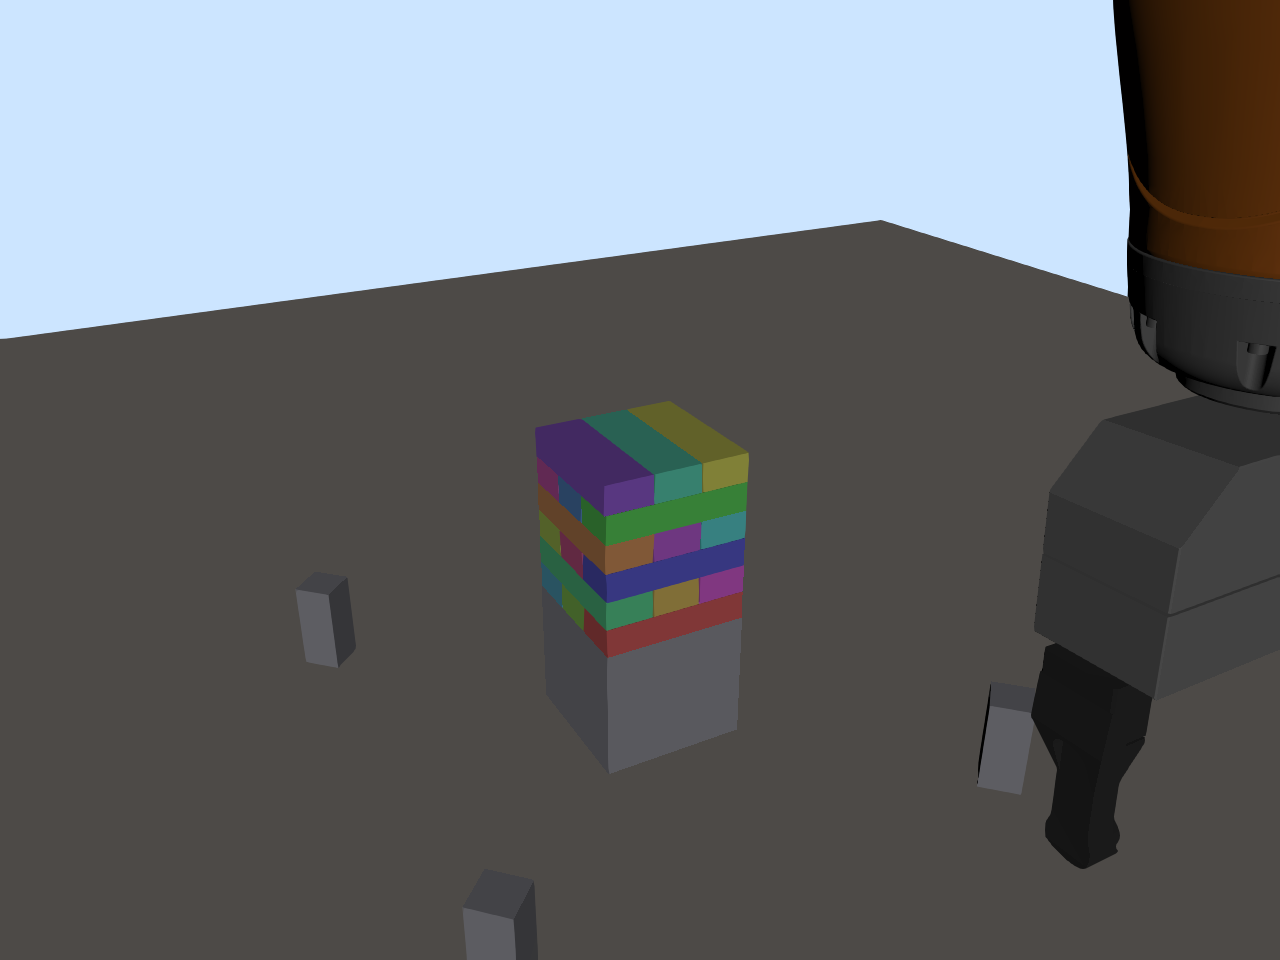
\includegraphics[width=0.48\linewidth]{figures/camera_base.png}\hfill
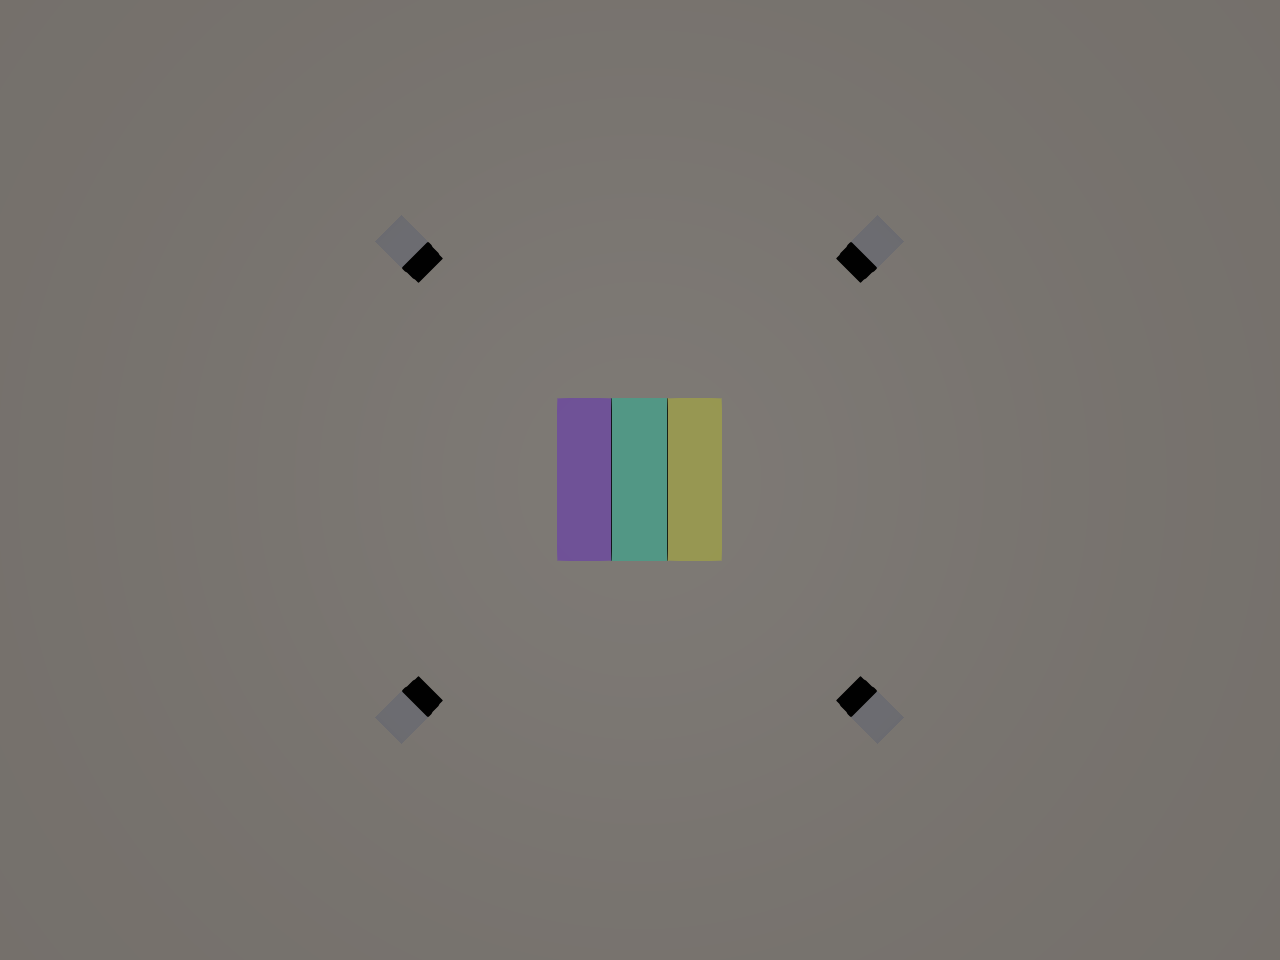
\includegraphics[width=0.48\linewidth]{figures/camera_top.png}
\caption{The two cameras' views of a fresh tower with one hue per block. Left: base camera (turns with the robot; the
gripper is at right, pedestals visible). Right: top camera, which sees only the top layer.}
\label{fig:cameras}
\end{figure}

% ======================================================================================================
\begin{thebibliography}{00}
% [TODO: verify every entry against the source before submitting]
\bibitem{fazeli2019} N.~Fazeli, M.~Oller, J.~Wu, Z.~Wu, J.~B.~Tenenbaum, and A.~Rodriguez, ``See, feel, act:
Hierarchical learning for complex manipulation skills with multisensory fusion,'' \textit{Science Robotics}, vol.~4,
no.~26, 2019.
\bibitem{besl1992} P.~J.~Besl and N.~D.~McKay, ``A method for registration of 3-D shapes,'' \textit{IEEE Trans.\
Pattern Anal.\ Mach.\ Intell.}, vol.~14, no.~2, pp.~239--256, 1992.
\bibitem{arun1987} K.~S.~Arun, T.~S.~Huang, and S.~D.~Blostein, ``Least-squares fitting of two 3-D point sets,''
\textit{IEEE Trans.\ Pattern Anal.\ Mach.\ Intell.}, vol.~PAMI-9, no.~5, pp.~698--700, 1987.
\bibitem{elandt2019} R.~Elandt, E.~Drumwright, M.~Sherman, and A.~Ruina, ``A pressure field model for fast, robust
approximation of net contact force and moment between nominally rigid objects,'' in \textit{Proc.\ IEEE/RSJ IROS},
2019.
\bibitem{tedrake_manip} R.~Tedrake, \textit{Robotic Manipulation: Perception, Planning, and Control}, course notes for
MIT 6.421/6.4210. [Online]. Available: \url{https://manipulation.csail.mit.edu}
\bibitem{drake} R.~Tedrake and the Drake Development Team, ``Drake: Model-based design and verification for robotics,''
2019. [Online]. Available: \url{https://drake.mit.edu}
\end{thebibliography}

% ======================================================================================================
\appendices
\section{Development Log: Problems, Causes and Fixes}\label{app:log}
% Every problem we traced, with the measured evidence (one game each on a Mac unless noted).  Check with the course
% whether appendices count toward words.
\subsection*{Simulation and control}
\begin{enumerate}
\item \textbf{The whole layer above slid out with a pulled block.} Per-leg and contact-force readouts ruled out a high
hand, a rolling block and uneven load (0.42\,N on the pulled block vs.\ 3.11\,N on its neighbours); once sliding started
the load shifted onto the pulled block. Switching Drake's SAP solver to ``lagged'' stopped it (0.2\,mm) (D-10).
\item \textbf{Fingers closed while the hand was already leaving}: a waypoint's finger command acts from the next leg.
Per-waypoint durations let a closing step be held (D-04).
\item \textbf{Replays changed results.} The continuous integrator was stepped by the simulator, which also stops at each
replay frame; trial 40 placed 6 blocks without a replay and 4 with. A discrete integrator (1\,ms substeps) made them
identical (D-24).
\item \textbf{Mac and cluster disagree on close calls.} The same code and Drake version replaced a block on the cluster
and dropped it on the Mac; floating-point differences decide marginal grasps, so we judge changes on the machine that
runs the results.
\item \textbf{Step size.} Moving the physics step from 1 to 5\,ms (for speed) flipped a marginal push turn from replaced
to dropped; at 1\,ms the picks and outcomes of a game matched, but per-turn disturbances were 1.3--9$\times$ larger, so
5\,ms ``mm moved'' figures are lower bounds.
\end{enumerate}
\subsection*{Pulling}
\begin{enumerate}\setcounter{enumi}{5}
\item \textbf{Pad height}: half the block width instead of height, 7.25\,mm high against a 0.875\,mm margin; a lift that
went down (sign of the hand's $z$ axis).
\item \textbf{Push-method pull dragged the tower} (worst block 70--230\,mm). Traced with per-block contact loads: the
block above loaded the pulled block more than its other supports and pushed its neighbour along. Tried: a fast pull
(13--16\,mm), a 0.4--1\,mm lift after gripping (overshot), deeper grips, an open-loop hand tilt ($\pm$0.4$^\circ$: worse).
Worked: a firmer squeeze (194$\to$5.3\,mm) and one smooth slow pull (2.7\,mm). Pull only with two or more layers on top.
\item \textbf{Edge blocks cannot be pushed}: an end push twists the crossing blocks above (11.4\,mm vs.\ 0.27\,mm for
end-pinch at six layers).
\item \textbf{End-pinch pull speed}: 1.0\,s collapsed a layer-4 pull; 0.1\,s moved the tower 1.6--2.6\,mm on layers 3--4.
The fast pull leaves the hand $\sim$12\,mm behind its target at the end of the leg.
\end{enumerate}
\subsection*{Regrab and carry}
\begin{enumerate}\setcounter{enumi}{9}
\item \textbf{Top-down regrab out of reach}: no IK solution at the 0.95\,m standoff (it would need $\sim$0.65\,m), and a
level hand cannot pick a block off the table; hence the pedestals (D-22).
\item \textbf{Regrab drifted 2--11\,mm as one motion} (feedforward controller) and dropped the block; a separate plan
starting with a joint move on the measured block fixed it (grasp error 0.7--3.6\,mm).
\item \textbf{The swing to the regrab knocked the block off the post.} A kinematic check of start heights (clearance
21.5\,mm at 0, 32.4 at 20\,mm, 66 at 50\,mm, with larger arm-shape changes above 20\,mm) picked 20\,mm; 30 and 50\,mm
failed on the cluster.
\item \textbf{The block slipped during the tuck} before placing (a $\sim$155$^\circ$ joint swing); no tuck before a place cut
the largest swing to 52$^\circ$ and the simulated turn time (O-5).
\end{enumerate}
\subsection*{Placing}
\begin{enumerate}\setcounter{enumi}{13}
\item \textbf{Middle slot between two edges}: collapse or 16\,mm off; middle first: the far edge hit it; outward-aimed
edges: removed. Adopted: edge, middle from the same station, edge.
\item \textbf{The block slides in the pads during the base's turn} (3--6\,mm): grasp correction, landing within 1\,mm (D-08).
\item \textbf{Releases dropped onto a lower tower}: built heights included a 0.5\,mm gap per layer that closes as the
tower settles (1.9--3.6\,mm drops on layers 6--8). Removing the gap raised early failures (Table~\ref{tab:gap}); a 1\,mm
release lift inside \texttt{plan\_place} was silently cancelled by the grasp correction. Kept the gap and aimed at the
measured top (D-25).
\item \textbf{Hand jumps $\sim$1.2\,mm when the fingers open} and the top two layers lurch $\sim$6\,mm on a layer-7 middle
place; nothing moves while the hand backs away. Not fixed.
\end{enumerate}
\subsection*{Strategy and statistics}
\begin{enumerate}\setcounter{enumi}{17}
\item \textbf{Early results were luck}: after 10 trials random averaged 2.2, over trials 10--49 3.3; at 50 trials no
difference was significant. We moved to 100 paired trials, fixed measures in advance, and confirmed on fresh trials.
\item \textbf{Identical collapse distances mean identical games} (the simulator is deterministic per pick sequence), so
11 early failures were 3--4 repeated situations.
\item \textbf{Weights}: preferring high layers pulled under a loaded top; preferring low weakened the base; clear-of-top
over two layers cost 0.60 blocks ($p=0.0002$); V2 won (Table~\ref{tab:strategy}).
\item \textbf{The 6-block ceiling} was the seventh pull toppling the tower, not the strategy; we did not tune on that one
game. Hollow columns ended 93\% of V2 games (O-8), fixed by the column filter.
\end{enumerate}
\subsection*{Perception}
\begin{enumerate}\setcounter{enumi}{21}
\item \textbf{Colours}: a six-colour scheme repeated once blocks moved; 18 hues identify every block (99\%); added
brightness or saturation levels confused shaded faces (49\%).
\item \textbf{ICP tests can mislead}: scene points on the model's own grid let ICP lock one grid step off (2--11\,mm);
random surface points gave 0.03\,mm.
\item \textbf{Middle layers 0.6--1.5\,mm high}: they show only end faces (94\% of block 9's points), so ICP stalled near
its built-height start; the settled-height start gave 0.31\,mm.
\item \textbf{Heights drifted over a game} (0.45$\to$1.04\,mm in 3 turns): ICP could not follow sags smaller than its
2\,mm model spacing; 0.5\,mm spacing (0.19$\to$0.58\,mm). Resetting the guess each turn did not help.
\item \textbf{A blended edge became a third block}: hues 160$^\circ$ and 260$^\circ$ blend to 220$^\circ$, block 13's; 99
such points put block 13 8\,mm high. Outlier rejection fixed it.
\item \textbf{In-hand guess}: assuming the end-pinch grasp missed the push grasp by 44\,mm; recording the grasp when the
fingers close works for any method (held block within 0.3\,mm).
\item \textbf{Cluster rendering}: the container lacked EGL; a smoke test caught it before 200 jobs ran.
\end{enumerate}
\owner{Seetha, Mitch}{add the probe, turntable and push-tuning problems you traced.}

\end{document}
